\chapter{Introduction}
    
    \section{Objective}
    
    Design the control for one degree of freedom of an exoskeleton using sEMG signals from the user as the input signal. To accomplish this goal, three different control methods will be designed, evaluated and compared to determine which  one is more accurate and more easily controlled by the user. The three evaluated control methods will be: a model-based control, a proportional control and a hybrid control using sEMG and force sensors.
    
    An available exoskeleton will be adapted and the designed exoskeleton control will be applied.	    
    
    
    \section{Bibliographic Revision}
    
    In the United States, the number of people between the age of 18 and 64 that has some kind of movement disability has increased about 12\% between the years 1981 and 2014 \cite{VonSchrader2017}. Two of the main causes for disability are stroke and spinal cord injury. Yearly, 15 million people suffer stroke. From these, 5 million are fatal and 5 million cause a permanent disability. These number have been increasing in recent years and studies indicate these numbers will increase even further \cite{mackay2004atlas}. From 250 thousand to 500 thousand people suffer spinal cord injury yearly. The three main causes for spinal cord injury are traffic accidents, falls and violence. The non-traumatic injuries have been increasing in recent years. Moreover, with the rising in life expectancy of the world population \cite{UN}, the number of people affected by movement disabilities that difficult movement also raised.

	Due to these factors, the need for mechanisms that assist human movements have become more important. One of these mechanisms is the robotic exoskeleton.
    
	They are electromechanical structures coupled to physiological limbs, capable of doing or assisting movements. A robotic exoskeleton is usually composed of joints and rigid bodies \cite{pons2008wearable}.
There are several biological signals that can be used to control an external device. For exoskeleton control, that has the goal of moving a certain limb, it is interesting to use the same signals that are present in the human body, like the neural control signals responsible to activate the muscles. Since these signals cannot be accessed directly, the use of electromyography (EMG) has been explored to control these devices.
	
    The surface electromyography (sEMG) signal represents the electrical activity generated in muscle fibers in response to the activation provided by innervating motor neurons. The information present in the EMG signals is a composition of the synaptic inputs received by the motor neurons and the electrical properties from the muscle fibers \cite{Farina1215}.
    
     There are several other approaches to the control of a mechanical limb apart from the EMG signal. Among the relevant methods, some have been used in combination with EMG for the control of the prostheses or ortheses.
    

\subsection{EMG Control}

    Battye, Nightingale and Whillis \cite{Battye506} first proposed the use of proportional EMG control. The authors developed an apparatus capable of performing open and close actions according to when the test subject performed a grasp with his fingers. The apparatus consisted of: electrodes attached to the skin of the forearm; an electrical amplifier; a discriminator, which powered a solenoid when input signal was detected; the solenoid activated a hook, closing it. As a result, the authors were capable of designing a control system sensitive enough to close, and remain closed, when the test subject gripped a pencil in the fingers, regardless of the movement of other limbs. This concluded that the signal captured by the apparatus successfully eliminated the EMG signal from other muscles.
	
    Bottomley et al. \cite{Bottomley411} proposed another method for EMG-driven prostheses control. Two EMG electrode channels were placed on the forearm, one on the hand extensors and another on the hand flexors, to measure the muscle activity.  The signal from the muscles were amplified, rectified and smoothed. To remove the “cross-talk”, that is, the influence of the neighbor muscles on the targeted muscle, the signal of the neighbor muscle is subtracted from the signal obtained from the target muscle. These signals were used to control a Split hook capable of grasping objects, that exerted a force proportional to the EMG signal intensity. To control the desired force, a force sensor was attached to the hook. This device included a feedback control system that was capable of increasing, or decreasing, the Split hook grasping force compared to the measured EMG signal. When the force sensor detected zero force, that is, the hook is not grasping the object anymore and it is freely moving, the intensity of the EMG signal controlled the speed of the hook. A backlash generator was introduced in the electrical system, attenuating random variations when the signal changes exceeded a preset limit, that widens as the force feedback signal increases. The authors state that, after a few minutes wearing the apparatus, all the test subjects, even amputees, were able to control the hook in a graded manner.
    
    Similarly, Alter \cite{alter1966bioelectric} designed an exoskeleton control using two differential electrodes, one on the biceps and one on the triceps. Both signals were rectified and then the triceps signal was subtracted from the biceps signal. An adjustable lowpass filter was implemented. This signal was used as input signal to a power amplifier that powers an electric motor. Strain gauges were attached to the exoskeleton for force measurement, and the signal obtained from the strain gauges entered the system as a feedback signal. 
    
    Isidori and Nicolo \cite{Isidori1966} first described the myopulse processing technique, which was later developed by Childress et al. \cite{childress1971} and Philipson \cite{Philipson1985}. The myopulse processor works as follows: when the absolute value of the EMG surpasses a predetermined threshold value, the output of the processor turns on. This way, whenever the EMG activity rises, the duty cycle of the myoprocessor output will also increase. An illustration of this method can be seen in figure \ref{Myopulse Processor}.
    
    \begin{figure}[t]
      \centering
      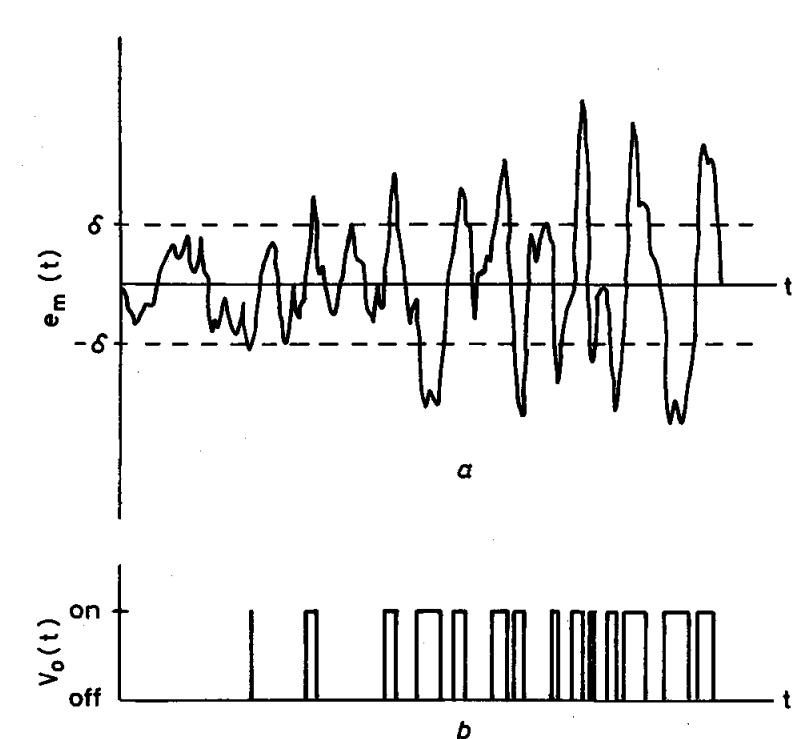
\includegraphics[scale=0.5]{Images/Myopulse.jpg}
      \caption{Illustration of the myopulse processing technique. The upper trace shows a typical bandpass-filtered EMG signal recorded with surface electrodes. The output will remain off as long as the absolute value of the EMG signal in the upper trace is below the level $\delta$, otherwise the output will be turned on. The lower trace illustrates the output from the myopulse processor \cite{Philipson1985}}
      \label{Myopulse Processor}
   \end{figure}
   
    In his system, two sets of electrodes were placed over the targeted muscle where the detection of electrical signal was desired. The EMG signal was sent to the myopulse processor, where the input signal was amplified and transformed into Pulse Width Modulated (PWM) signal. This PWM signal was sent to the microcomputer. Then, the microcomputer processed the PWM signals and sent the output signals to control the prosthetic arm according to the control algorithm. The myopulse processor is an electrical circuit composed of a dual comparator, with the value of the resistors defining the threshold value $\delta$.
    
    The signal measured through the EMG electrode is an analog signal, since it is a measure of the electrical activity of the muscle. To use this signal in a controller, it is needed to convert this signal to a digital signal.
    One advantage of this system is that, with the myopulse processor, there is no need for a conventional analog-to-digital converter. 
    The author also implemented a classification method for the prosthesis control. Different from the previous control methods, where the actuation of the joint was proportional to the intensity of EMG signal, this system can perform different movements. In this work, by measuring the intensity of EMG signals from two electrode sets, the author was capable of achieving seven different movements. Figure \ref{Movement space} shows the proposed dynamic area for the prostheses control. According to the intensity of the input from the two target muscles one of the seven possible actions is performed.
    This control system was applied to a prostheses and tested on four amputees subjects. With proper training sessions, the amputees were able to perform some daily tasks such as grasping a plastic cup containing water, pour the desired amount and then release the cup. In the case of the nonamputees, the subjects could achieve good control over the seven-state control system. 
    
    \begin{figure}[thpb]
      \centering
      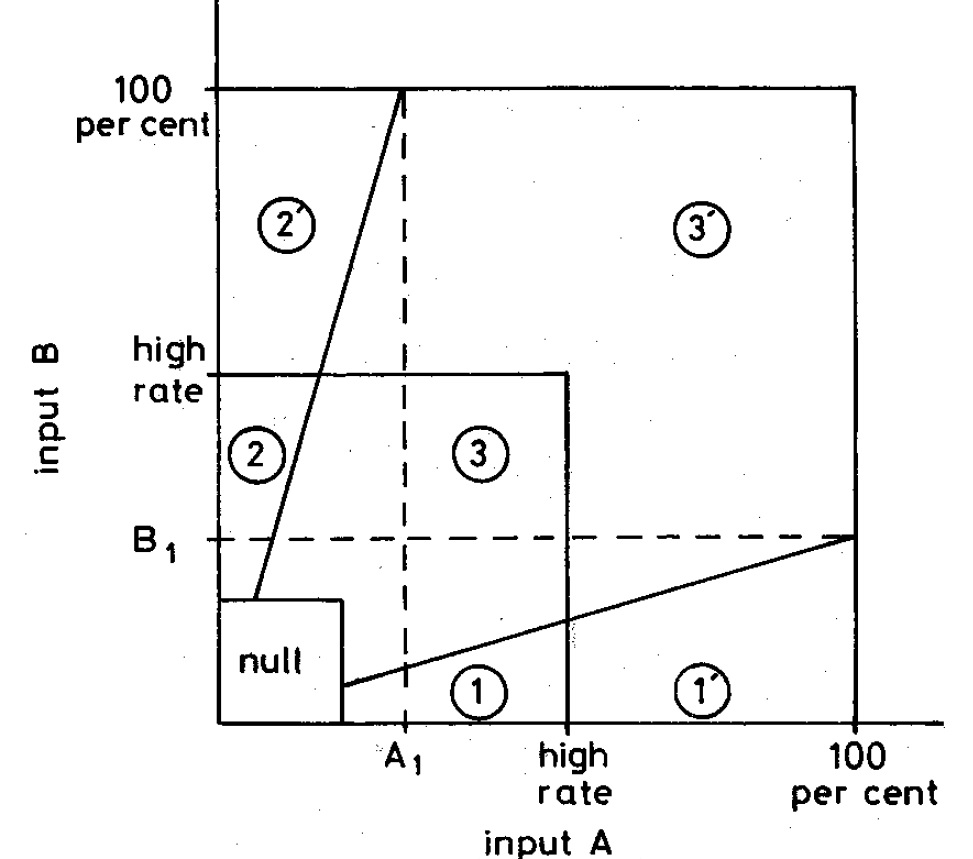
\includegraphics[scale=0.5]{Images/Movement_Area_-_Philipson.jpg}
      \caption{Diagram showing the possible movement areas according to the muscle inputs \cite{Philipson1985}}
      \label{Movement space}
   \end{figure}
   
   Parker et al. \cite{Parker1977662} sought to develop a better processor for the EMG signal, that is, find the signal processor that achieves the minimum error at selecting the desired action for the prostheses. The authors developed a model that extracts the relevant information from the myoelectric signal obtained by a bipolar electrode configuration. One of the main points of this model is that the pooled motor unit firing rate reflects the contraction level and is thus the information parameter in the myoelectric signal. Hogan \cite{4123279,4123280}, also in search of a better myoprocessor, developed a similar mathematical model to estimate muscle force based on EMG signal. 
    
    The myoelectric signal is a zero-mean stochastic process. To estimate the user's control signal, it is necessary to add a nonlinearity to the estimator. Typically, a full-wave rectifier is used for this nonlinearity, followed by a low pass filter. Evans et al. \cite{4121805} proposed another model based approach to this EMG control problem. The authors used a logarithmic nonlinearity, followed by a a linear minimun mean-square error in the EMG-force estimation. This way it was possible to add a Kalman filter to estimate the control signal. 
    
     Hudgins \cite{Hudgins204774} proposed a control strategy for a multifunction prosthesis based on the classification of myoelectric patterns into different movements. Initially, the author conducted tests on both healthy subjects and amputees. The test consisted of an isometric contraction with constant force and a contraction (e.g. flexion, extension, etc.) with no constraints related to force, velocity or range. The subjects were asked only to make consistent motions, starting from a comfortable neutral position.
     
     By taking the average of the EMG signal for the first 300ms to 600ms of the movement, that is, the onset of the movement, it was possible to detect different signal patterns for each movement (e.g. elbow flexion, elbow extension, forearm supination, etc.) shown in figure \ref{EMG patterns}. Other control schemes, based on steady state levels, are limited to only three limb functions: for an elbow mechanism, one can only control extension, flexion and the off-state. The scheme proposed by Hudgins targets the EMG signal of only one muscle and is capable of assigning as many functions as the number of distinct signal patterns generated by the muscle.
     
         \begin{figure}[thpb]
      \centering
      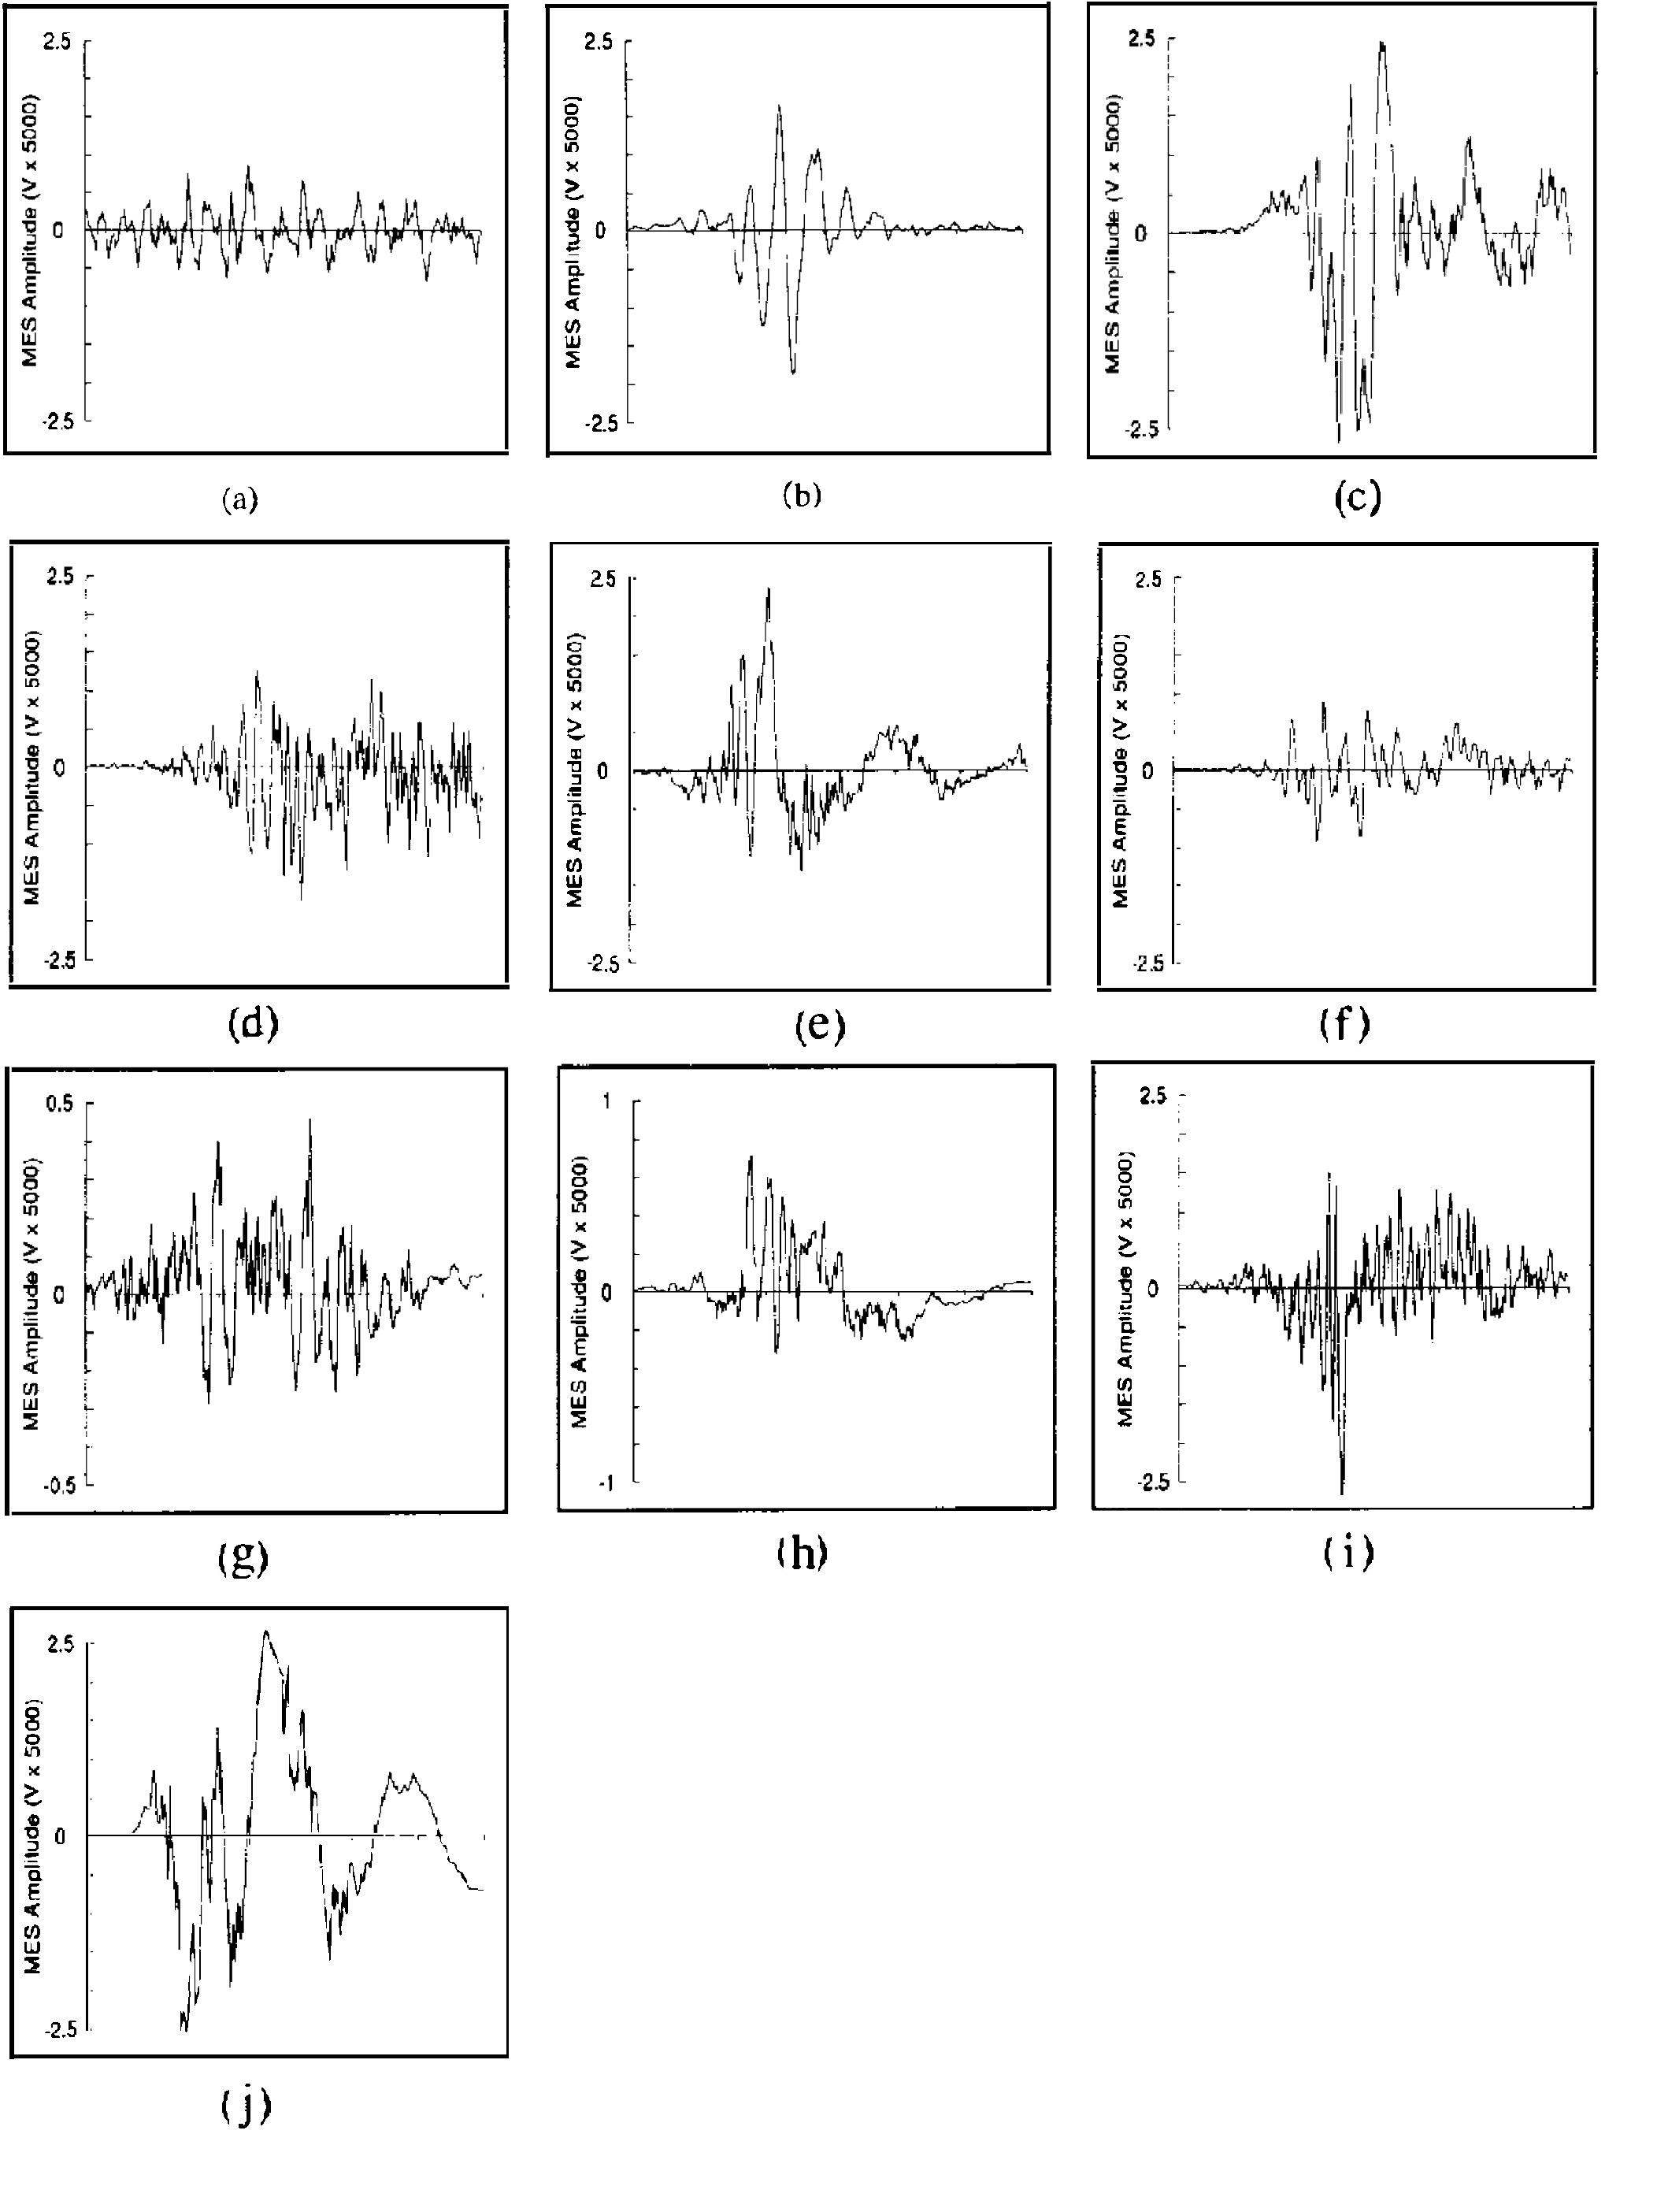
\includegraphics[width = \textwidth]{Images/EMG_patterns.jpg}
      \caption{Average of the first 300ms of the EMG recordings for the following movements: For a normally limbed subject: a) Isometric contraction; b) elbow flexion; c) Forearm supination; d) elbow extension; e) wrist flexion; f) forearm pronation; for the amputee subject: g) inward humeral rotation; h) contraction of the flexor muscle group; i) contraction of the extensor muscle group and j) biceps/triceps co-contraction. Adapted from \cite{Hudgins204774}}
      \label{EMG patterns}
   \end{figure}
   
   Since the prosthesis is capable of performing different movements, it is necessary to implement a classifier, that is, a method that chooses the desired movement or action based on the input signal. An Artificial Neural Network (ANN) was chosen as the classifier. The authors proposed a group of parameters, called features, which served as input to the classifier. The following features were chosen to represent the myoelectric patterns: Mean Absolute Value (MAV): it is the mean value of the signal throughout the data segment; Mean Absolute Value Slope: is the difference between the MAV of each segment; Zero Crossing (ZC): number of times the waveform crosses the zero value (it is needed to add a "dead-zone" to the signal to avoid noise inducted zero crossings); Slope Sign Changes (SSN): the number of times the slope of the waveform changes sign (the same "dead-zone" applied previously must be applied here); Waveform Length (WL): is the cumulative length of the waveform throughout the data segment. By using these previous features, one can get values for waveform amplitude, frequency and duration within a single parameter. This classification method has become known as the Time Domain feature set \cite{Johnny2009}.
   
   Tests showed that the subjects were capable of performing up to four different movements with an accuracy ranging from 70-95\%, before training. However, a major drawback from this control scheme is that, since the classification method only considers the movement onset, the EMG signal must always start from a resting position. If the user tries to switch from one movement to another in a period of time smaller then the averaging window (300ms-600ms), the control scheme will fail.
   
   Englehart \cite{Englehart1999431}, further developing the pattern recognition problem, tested some time-frequency-domain sets  for the EMG signal processing. The sets used were: Short-time Fourier Transform (STFT), Wavelet Transform (WT) and Wavelet Packet transform (WPT).
   
   The same group also proposed a method  to overcome the previous problem regarding the fast transition between two different movements \cite{Englehart1206493}. To do so, instead of segmenting the EMG data into multiple frames for classification, now the data was acquired continuously on a single, unsegmented window. In this scenario, the data acquired from 12 subjects were compared using the Time Domain statistics and using the time-frequency-domain sets. The Time Domain sets outperformed the time-frequency-domain sets in continuous data acquisition.
   
   Jiang \cite{Jiang4663628} proposed a method to estimate force from the Mean Square Value (MSV) of the EMG signal. MSV is defined as the mean value of the square of the signal throughout the data segment. By stating that it is possible to maintain the muscle cross-talk at low levels, it is possible to determine a direct relationship between muscle force and sEMG measurements.
   
   \subsection{Hybrid Control and Other Control Modalities}
   
   \subsubsection{Hybrid Control}
     
   If the subject had some residual shoulder movement it is possible to combine a joystick at the shoulder with EMG for a movement classification method \cite{Losier4353750}. The system was capable of performing nine different activities. Eight of then were controlled by the position of the shoulder and one by EMG input when the user performed a humeral rotation movement. The Time Domain technique was used to differentiate the EMG readings from humeral rotation from the normal shoulder movements.
   
   Fougner and Stadvahl \cite{Fougner2008}\cite{Fougner2011} used force sensors on the EMG electrodes to measure external forces. This application is useful for the cancellation of artifacts caused by these forces (e.g. movement artifacts). 
   
   Fougner \cite{Fougner5985538} noted that different limb positions associated with daily activities can affect the EMG signal results. To overcome this problem, the EMG signal was associated with accelerometers placed at the user's forearm and biceps. This allows the pattern recognition system to know the position and orientation of the limb, compensating for eventual changes on the EMG signal.
   
   \subsubsection{Other Control Modalities}
   
   If EMG sensors are difficult to place or cause discomfort to the user it is possible to use other techniques like Mechanomyography (MMG). Silva \cite{Silva1280527} used MMG for a classification method control strategy. Mechanomyography is the measurement of the mechanical vibrations caused by the contraction of the muscle. In this case, the MMG sensors were used as a substitute of the EMG sensors, when the EMG sensors are of difficult placement or unconfortable for the patient. This method can also be referred as phonomyogram, vibromyogram, soundmyogram or acoustomyogram, since the sensor is composed of a microphone and an accelerometer that detect the air vibration between the sensor and the target muscle. 
   
   Kenney \cite{Kenney1999589} used the dimensional change of the muscle as control signal for his control strategy. This technique is called Myokinemetric. The author designed a sensor, composed by a Hall Effect sensor and a permanent magnet. The relative distance between these two components varied according to the dimensional change of the subject's muscle. To validate this strategy a tracking test was performed, where the test subject was supposed to track a signal presented on a screen by controlling the dimension of his muscle.
   
   Stadvahl \cite{Standvahl1997} used ultrasound to create a force estimation. As the muscle contracts, the shape of the muscle changes. The ultrasound, when transmitted to a medium, generates an echo signal that can be acquired through an ultrasound sensor. Using this information, it is possible to determine a relation between the ultrasound and the force through the Cross Correlation technique. Chen \cite{Chen2011} attached ultrasound transducers to the subject's forearm to estimate the wrist angle using the ultrasound signal. 
   
   Nightingale \cite{NIGHTINGALE1985167} used force and slip sensors on the Southampton Hand to detect forces applied to the hand and relative slipping motion between the hand and objects. By using the force and slip sensors paired with an EMG control, state machine control logic could be implemented. According to the EMG signal magnitude the control logic would open or close the hand and through the force sensors measurement it was possible to asses more specific states for the hand movement, like holding or squeezing an object.
   
   \subsection{State-of-the-Art of Exoskeletons and Exoskeleton Control}
   
   The exoskeletons can be divided according to their applications: performance enhancement, haptic interfaces, remote operation, functional assistance (active orthoses and prostheses), rehabilitation and motor control exploration. In this work two groups will be focused: the performance enhancement and the functional assistance. The performance enhancement exoskeleton allows healthy users to perform a difficult task by either reducing the forces or the expended energy, or perform a task that is impossible to accomplish by human strength or skill, solely. The functional assistance assists the user by modifying or recovering the motor function of the neuromuscular and skeletal system. However, this distinction, in some cases, can be not as clear \cite{Dollar4456745}.
   
   One of the major incentives to the development of exoskeleton has been the Exoskeletons for Human Performance Augmentation (EHPA), a program supported by the Defense Advanced Project Agency (DARPA). This program is developing exoskeletons capable of increasing the capabilities of ground soldiers beyond that of a human. There are three critical technologies that are the focus of this program: Energy, power and actuation; controls and haptic interface; design and integration \cite{Ephraim2002822}.
   
   HAL (Hybrid Assistive Limb) is an exoskeleton focused on both performance-augmenting as well as rehabilitation \cite{Sankai2011}. The HAL-5 is a full-body exoskeleton. The joints are powered by DC motors with harmonic drives placed directly on the joints. Attached to the exoskeleton is an special shoe with ground reaction force sensors. It is attached to the user by harnesses at the hip, thighs, calves, upper arms and forearms, as well as the shoe. 
   
   The HAL-5 utilizes a broad range of sensors for its controlling. The intention detection is done primarily by sEMG sensors. As soon as the EMG level exceeds a threshold, the motion support is triggered. An assistive torque is provided to the user. This torque is composed of three parts: an assistive torque; a viscous torque that prevents high velocity motions, maintaining safety; and a gravity compensating torque \cite{kawamoto2010}. In some experiments, the motion intention detection was done by the ground reaction sensor, to adapt the exoskeleton for patients with spinal cord injury. When the user shifts its weight to the next stance leg, the reaction force on this leg is higher that the other, triggering the exoskeleton motion \cite{Tsukahara2015}. Also, there are potentiometers, gyroscopes and accelerometers for the measurement of the angle, speed and acceleration of limbs and joints.
   
   \begin{figure}[thpb]
      \centering
      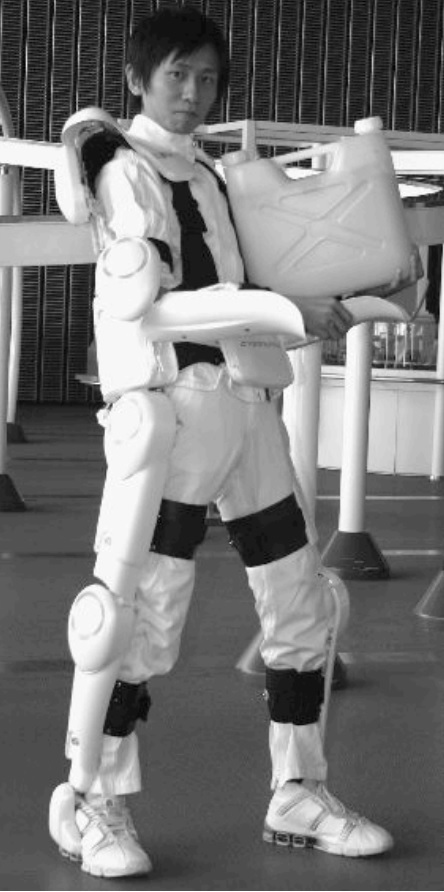
\includegraphics[scale=0.4]{Images/HAL5.jpg}
      \caption{HAL-5 exoskeleton \cite{Sankai2011}}
      \label{HAL5}
   \end{figure}
   
   In \cite{Otsuka6181399} the authors further developed the HAL upper-limb exoskeleton for meal assistance. It is composed of a shoulder joint with three degrees of freedom and an elbow joint with one degree of freedom. Also, a grasp assistance mechanism is attached to the forearm to allow for manipulation of objects by the user.
   
   One interesting aspect of the HAL exoskeleton is its modularity. Currently, there are separated products for upper-limbs, lower-limbs, lumbar support, as well as other modalities, like a heavy-duty and a disaster recovery exoskeleton \cite{cyberdyne}.
   
   The manufacturer states that the full-body HAL-5 weighs approximately 23kg, has a continuous operating time of approximately 2 hours and 40 minutes and is capable of lifting objects up to 70kg. The HAL\textsuperscript{\textregistered} exoskeleton is capable of performing different activities such as standing up from a chair, walking and climbing up and down stairs.
   
   The HAL\textsuperscript{\textregistered} exoskeleton is already used in many medical institutions in Japan and already received certification for clinical use in Europe. It is commercialized by Cyberdyne Inc.   
   
   
   
   The Berkeley Lower Extremity Exoskeleton (BLEEX), funded by the DARPA, is a self-powered exoskeleton that enhances the strength and endurance of a human \cite{Kazerooni2006}. 
   
   \begin{figure}[thpb]
      \centering
      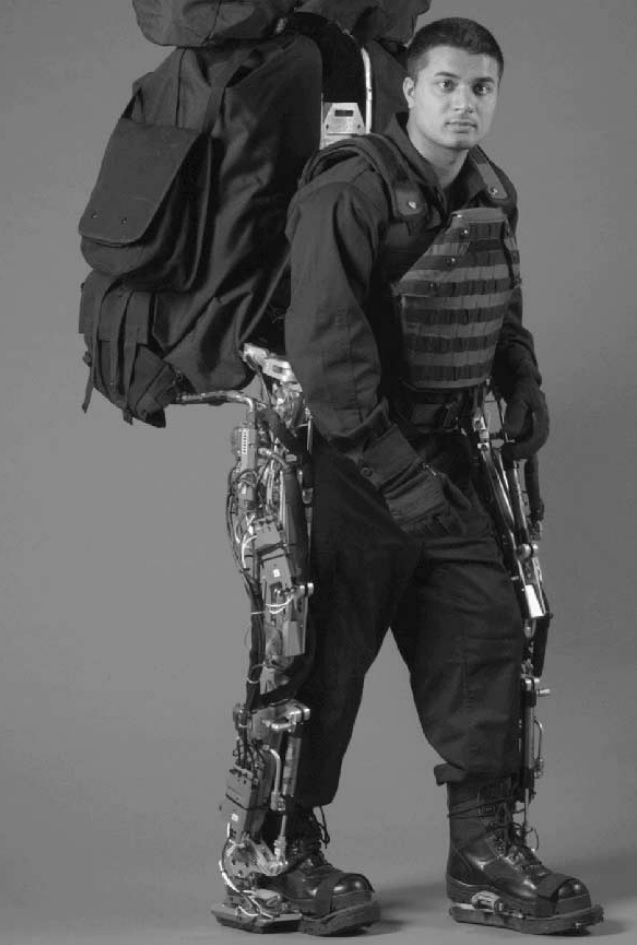
\includegraphics[scale=0.4]{Images/BLEEX.jpg}
      \caption{University of California at Berkeley's BLEEX exoskeleton \cite{Zoss1618670}}
      \label{BLEEX}
   \end{figure}
   
   The BLEEX exoskeleton has 7 degrees of freedom (DOF) per leg: 3 DOF at the hip, 1 DOF at the knee and 3 DOF at the ankle. For the hip, both the flexion/extension and the abduction/adduction joints are aligned to the human joint, but the rotation joint is positioned behind the user and under the torso. The reason is that, an aligned rotation joint would result in limited ranges of motion and singularities in some of the human postures. For the ankle, the flexion/extension axis coincides with the human ankle joint, but the abduction/adduction and rotation axis do not coincide with the human joint axis and form a plane outside of the human's foot. The front of the foot is compliant, allowing the flexing of the user's toes. The exoskeleton is only rigidly connected to the user at the hip and the foot \cite{Zoss1618670}.
   
   The BLEEX structure and actuation was designed based on the clinical gait analysis (CGA) of an 75-kg person. Analyzing the CGA, it was possible to determine which exoskeleton joint required actuation, based on the joint torque and power during gait. From this analysis, it was determined that the flexion/extension joints of hip, knee and ankle and the abduction/adduction joint should be actuated. 
   
   Initially, the selected actuator for the BLEEX was double-acting linear hydraulic actuators. They are compact in size, low weight and capable of exerting high forces. The actuators are placed in a triangular disposition in relation to the joint, resulting in a torque that varies according to the joint angle \cite{Chu1570789}.
   
   The average power consumption of the BLEEX during the walking cycle is 1143 W, compared to 165 W of mechanical power exerted by the human during normal gait. This exoskeleton is capable of supporting up to 75 kg and walk at speeds up to 1.3 m/s.
   
   In a later study, it was analyzed the feasibility of using electrical motors instead of the previous hydraulic ones. The designed electrical motors weighed an average of 4.1 kg opposed to the 2.1 kg hydraulic actuators. While the electric actuator weight is all centered in the actual joint, about 40\% of the weight hydraulic actuator is located away from the joint. At test performed at ground-level walking at the speed of 1.3 m/s, it was measured that the actuator power consumption was 598 W. Comparing both actuators, the electrical actuator is 95\% heavier and 92\% more power efficient \cite{Zoss2006}.
   
   An hybrid Hydraulic-Electric Power unit (HEPU) was designed in the attempt to provide autonomous energy for the exoskeleton. The hydraulic energy would supply the necessary mechanical parts of the exoskeleton, while the electrical energy would power the computer, sensors and other peripherals. Even though the designed HEPU could provide the necessary requirements of electrical and hydraulic power, it exceeded in both weight and noise output. The desired weight and noise output were 23 kg and 78 dBA, respectively. The achieved values were 30 kg and 87 dBA \cite{Amundson2006DevelopmentOH}.
   
   The control of the BLEEX exoskeleton has no sensors attached to the user. Every sensor is located only on the exoskeleton. It uses the forces applied by the environment and the user to the exoskeleton as the control signal \cite{Steger1642232}. The inverse dynamics of the exoskeleton are used as a feedback so that, when accounting the user force, the control loop gain approaches an unitary value. This control strategy has two main advantages: it allows for wide bandwidth maneuvers, necessary since the exoskeleton needs to respond to a wide variety of the human's movements; it is independent to changes in the user dynamics. The tradeoff of this control strategy is that it needs an accurate model of the exoskeleton dynamics. To address this, experiments in \cite{Ghan1642233} applied system identification methods to calculate the exoskeleton dynamics.
   
   One of the most well-established exoskeletons for disabled users is the ReWalk\textsuperscript{TM}. The ReWalk\textsuperscript{TM} is a lower extremity, battery powered exoskeleton that allows individuals with thoracic or lower level motor complete spinal cord injury to walk independently. It is suitable for adults who have preserved bilateral upper extremity function. The user must be using crutches to maintain balance. The mechanical structure is composed of bilateral supports parallel to the thighs and legs, articulated at the knee and hip. A rigid shoe insert fixes the user's feet. Velcro closures distributed at the legs and thighs and a waist belt secure the attachment between user and exoskeleton. The computer-based controller and the batteries are stored within a backpack. A tilt sensor is placed at the exoskeleton structure, near the waist \cite{Esquenazi2013}.
   
   The active joints of the ReWalk\textsuperscript{TM} are the knee and waist joint. The ankle joint is passive joint with spring-assisted dorsiflexion. The exoskeleton has five different operation modes. walk, sit-stand, stand-sit, up steps and down steps. In the 'walk' mode, the stepping procedure is triggered by the forward flexion of the upper body, measured by the tilt sensor. The maximum walking velocity is 2.2 km/h. The mode selection can be made through an user-operated wrist pad. There is also the option to manually control the position of the lower limbs \cite{Zeilig2012}. 
   
   \begin{figure}[thpb]
      \centering
      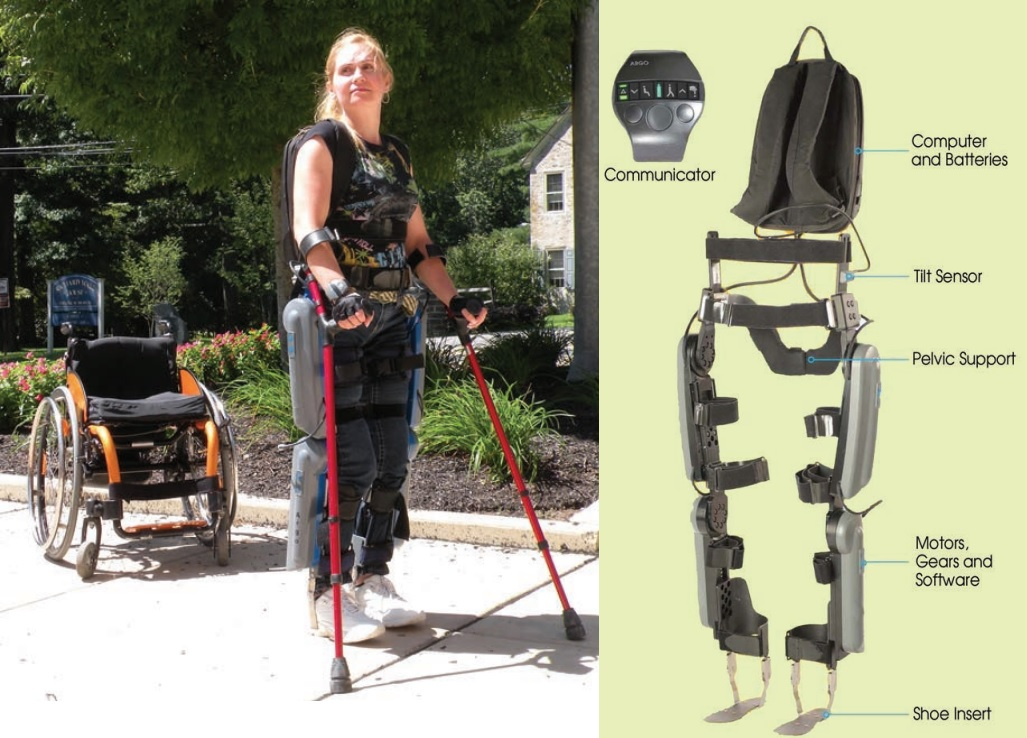
\includegraphics[scale=0.5]{Images/ReWalk.jpg}
      \caption{The ReWalk\textsuperscript{TM} exoskeleton worn by an user and its basic structure \cite{Esquenazi2013}}
      \label{ReWalk}
   \end{figure}
   
   Some studies have been performed with the ReWalk\textsuperscript{TM} \cite{Zeilig2012} \cite{Fineberg2013} \cite{Talaty6650469}. Overall the participants of the test were satisfied with the device, being able to walk without falling. The volunteers reached the level of being able to walk 100m with the use of crutches. However, they have not attained proficiency to use the device on a daily basis. It is stated that the users found relative difficulty with wearing and adjusting the device.   
   
   Even tough many advancements in this area have been made, the effective use of an exoskeleton continues to be extremely difficult. Even though many technologies have been advertised lately, there is a lack of quantitative studies available to researchers \cite{Young7393837}.
   
   The MIT exoskeleton, a quasi passive exoskeleton concept, explores the passive dynamics of human walking trying to achieve a lighter and more efficient exoskeleton. Although, tests performed show that the total metabolic cost of walking increased when used the exoskeleton while carrying a load, compared to no exoskeleton being used while carrying the load in a backpack. The increase in metabolic cost was found to be 10\% higher  \cite{Walsh2007}. Although, test participants stated that carrying the load while wearing the exoskeleton was more comfortable compared to carrying the backpack alone \cite{Valiente2005}. Another study demonstrated the exoskeleton is capable of transferring up to 90\% of the load to the ground, depending on the gait phase, but increases the metabolic cost in a range from 32\% up to 74\%, depending on some variations of the mechanical structure and actuation of the exoskeleton \cite{Walsh2006}.
   
   It has been previously studied that one of the major problems of ambulation devices for paraplegics is the high-energy demands imposed to the user. Franceschini et al. \cite{FRANCESCHINI1997582} conducted a survey on patients that utilized reciprocating orthoses (ARGO, RGO, HGO). From the 74 patients, 24 patients abandoned the use of the mechanism by the end of the study. One of the main reasons was the excessive energy cost.